\section{Implementación de bloques del sistema}

%COMENTARIO: ACÁ SE ME OCURRE DE HACER UNA INTRODUCCIÓN A CADA BLOQUE DEL SISTEMA, JUSTIFICAR Y EXPLICAR MEDIO POR ARRIOBA Y EN LAS SIGUIENTES SECCIONES EXPLICAR LOS DETALLES MÁS TÉCNICOS DE CADA BLOQUE.

En base a lo estudiado en la etapa de investigación, se pudo concluir que un sistema de captura de movimiento de las características necesarias para cumplir el objetivo del proyecto debe estar formado por 4 bloques generales: \emph{calibración}, \emph{detección de marcadores}, \emph{recontrucción} y \emph{seguimiento}. En la figura \ref{bloquesSist} se muestra un esquema del sistema a implementar.

\begin{figure}[H]
\begin{center}
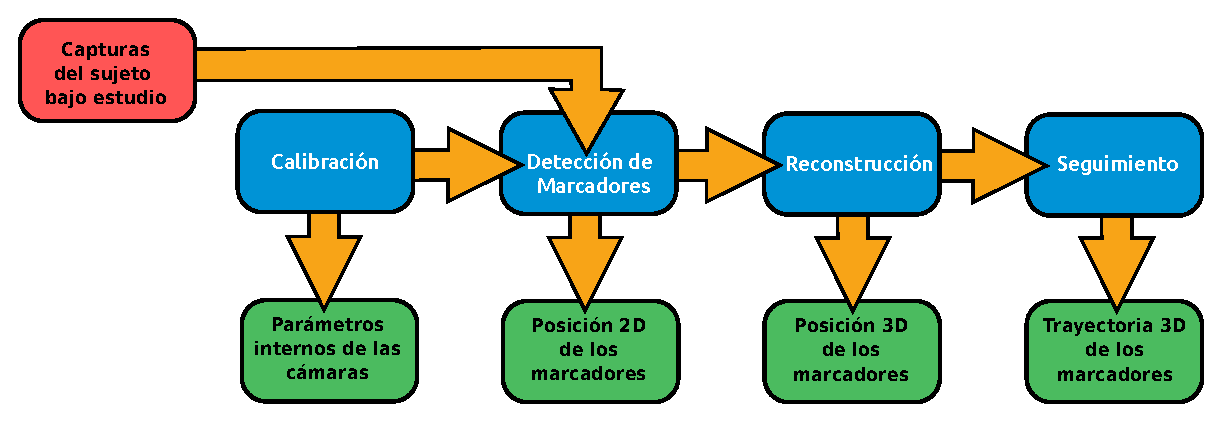
\includegraphics[scale=0.8]{img/Sistema_completo/Diagrama_de_bloques.eps}
\end{center}
\caption{Diagrama de bloques del sistema completo.}
\label{bloquesSist}
\end{figure}

A grandes rasgos, el sistema funciona de la siguiente manera:

\begin{enumerate}
	\item Se \emph{calibran} las cámaras. Esto es, determinar los parámetros de las mismas de forma tal de tener un mapeo del espacio 3D a las coordenadas 2D de las imágenes capturadas.
	\item Se realiza la captura del paciente en movimiento desde todas las cámaras calibradas.
	\item A partir de las secuencias, se realiza la \emph{detección de marcadores} para cada cámara. Esto equivale a determinar la posición 2D de dichos marcadores en cada cámara donde están visibles, a lo largo de toda la secuencia.
	\item Luego, con la posición 2D de determinado marcador en al menos 2 cámaras se realiza la \emph{reconstrucción} del mismo, es decir, obtener las coordenadas 3D de dicho marcador. Se realiza para todos los marcadores, y para todos los cuadros de la secuencia.
	\item Finalmente, se realiza el \emph{seguimiento} (o \emph{tracking}) de cada marcador en el espacio. Con esto se obtienen las trayectorias 3D de todos los marcadores en el cuerpo del paciente.
\end{enumerate}

Debido a los tiempos disponibles para realizar el proyecto en toda su magnitud, y a la planificación realizada al comienzo del mismo, la idea principal que se manejó en todo momento fue conseguir una implementación de un sistema con características similares, previamente elaborada, y adaptarlo para cumplir los objetivos establecidos. 

Sin embargo en la investigación bibliográfica se encontró otra realidad, ya que no hay muchos sistemas a disposición. Por un lado, la mayor parte de los sistemas encontrados están bajo costo de lisenciamiento (por ejemplo Vicon\footnote{http://www.vicon.com/, Noviembre 2014}, OptiTrack\footnote{http://www.naturalpoint.com/optitrack/, Noviembre 2014}, PhaseSpace\footnote{http://www.phasespace.com/index.html, Noviembre 2014}, Qualisys\footnote{http://www.qualisys.com/, Noviembre 2014} o MotionAnalysis\footnote{http://www.motionanalysis.com/index.html, Noviembre 2014}) y por otro lado, los sistemas Open Source que se encontraron no se adaptaban a las necesidades presentes o el trabajo a realizar era más costozo que hacer una implementación propia. Este último caso es el caso de Kinovea\footnote{http://www.kinovea.org/, Noviembre 2014}, que realizaba únicamente el seguimiento en coordenadas 2D.

Debido a los inconvenientes planteados, se decidió realizar una implementación propia de los bloques del sistema. Nuevamente, de acuerdo a la filosofía explicada en los párrafos anteriores, se priorizó la búsqueda de algun sistema ya diseñado para implementar antes de recurrir a la creación de uno.

Además, se tuvo presente para esta búsqueda el hecho de poder separar el sistema en bloques independientes. Esto asegura que la construcción de un bloque no quede a la espera del correcto funcionamiento de otro. Además, da la posibilidad de que en etapas futuras, se pueda realizar el estudio de uno de los bloques de la figura \ref{bloquesSist} en particular y asi poder modificarlo u optimizarlo a gusto. Esta forma de trabajo funciona adecuadamente siempre y cuando la salida de un bloque sea exactamente la entrada del siguiente, para los casos en que no se logró esto, se realizaron algoritmos capaces de importar la salida de un bloque y convertirla al formato de entrada de otro (por ejemplo, \textit{Xml2Struct} que convierte el xml que devuelve el bloque de detección de marcadores en estructuras de matlab para realizar la reconstrucción).

En la búsqueda realizada, se dió con la tesis de doctorado de Lorna Herda\cite{herda}, donde plantea un sistema de captura de movimiento de las características buscadas para este proyecto. Al estudiar dicho sistema se encontró que se encuentra bajo las mismas hipótesis de uso que el estudio preliminar realizado (utilización en fisioterapia, biomecánica, animación, deporte, etc.). Además, se encontraron muchas menciones de este trabajo en otros artículos de la misma rama científica y se encontró una documentación muy amplia respecto a la metodología y a su forma de implementarla. Por otro lado, si bien en todas sus menciones la metodología de procesamiento de datos es la misma, los bloques de calibración y detección de marcadores fueron variando.

Debido a las ventajas que presenta esta metodología respecto a las otras encontradas, se decidió por implementar este sistema e implementar los blqoues de calibración y detección de marcadores por otro lado.

Luego de estudiado el diseño de este sistema, se construyó un diagrama de bloques completo, más detallado que el mostrado anteriormente, que se puede observar en la figura \ref{diagBloq}. Es importante destacar que, si bien la mayor parte de los bloques de reconstrucción y tracking se realizaron con la metodología del sistema de Lorna Herda\cite{herda}, en la documentación se presentan ciertas ambigüedades en la descripción de algunos métodos y en la forma de actuar respecto a determinadas situaciones, que tuvieron que ser definidas por el equipo del proyecto en base a los conocimientos adquiridos.

A continuación se muestra el diagrama de bloques y se explica su funcionamiento.

\subsection{Diagrama de bloques}

\begin{figure}[H]
\begin{center}
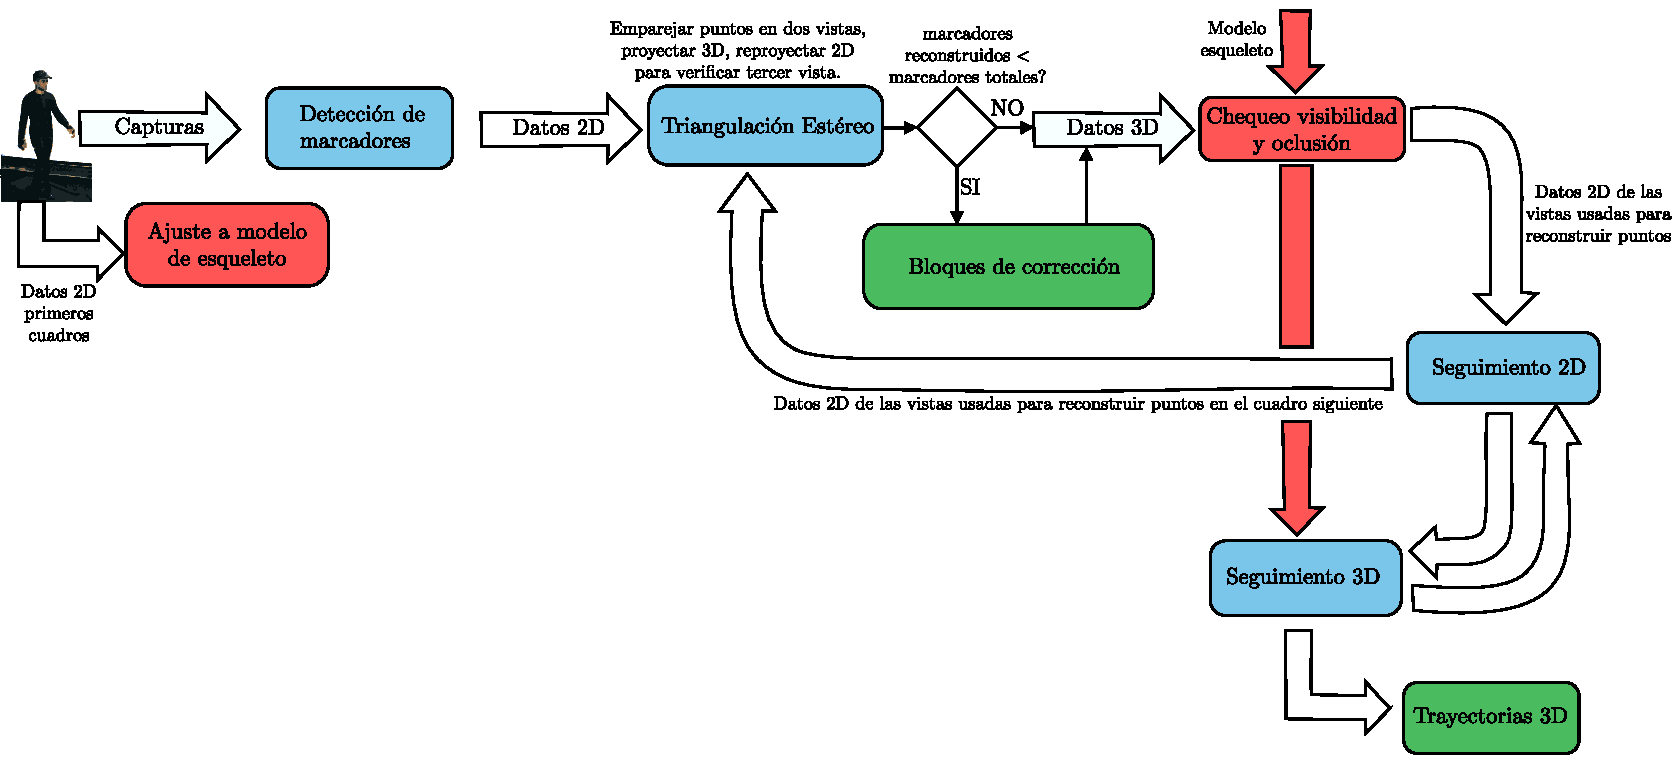
\includegraphics[scale=0.32]{img/Sistema_completo/Diagramadebloques_Herda.pdf}
\end{center}
\caption{Diagrama de bloques detallado del sistema.}
\label{diagBloq}
\end{figure}

En la figura \ref{diagBloq} se observa el diagrama completo del sistema a realizar, el mismo funciona de la siguiente manera:
\begin{enumerate}
\item Se realiza la captura de movimiento del paciente desde múltiples vistas, en un entorno controlado. Estas capturas son la entrada principal al sistema.
\item A partir de las capturas, por un lado se ajusta el \textbf{modelo teórico de esqueleto} a utilizar de acuerdo a las características del cuerpo del paciente, y por otro lado se realiza la \textbf{detección de marcadores} de cada cuadro para cada cámara. Este bloque es el mismo que el del diagrama de la figura \ref{bloquesSist} y se explicará en detalle en la sección \ref{deteccionMarcadoresSec}.
\item Luego que se tiene la posición 2D de los marcadores en cada cuadro y en cada cámara, se realiza la \textbf{triangulación estéreo} para obtener la posición 3D de los mismos. A grandes rasgos, la \emph{triangulación 3D} empareja dos puntos de dos vistas distintas y con ellos calcula la proyección 3D de ese punto en el espacio, luego se reproyecta ese punto en las otras vistas para verificar. Si verifica en al menos una vista más, entonces la posición 3D se considera válida.
\item Si el número de marcadores reconstruidos en 3D es menor al número total de marcadores en el modelo de captura, se ingresa en el \textbf{bloque de corrección}, donde se utilizan varios métodos para recuperar la posición 3D de los marcadores restantes (ver figura \ref{fig:bloqCorr}). 
\item Cuando se tiene la posición 3D de todos los marcadores, se ingresa en el bloque de \textbf{chequeo de visibilidad y oclusión} donde se verifica que la posición reconstruida de cada marcador sea correcta y no se haya reconstruido alguno con datos erróneos.
\item Finalmente, se realiza el \textbf{tracking 3D y 2D} en simultáneo para reconstruir las trayectorias de cada marcador.
\end{enumerate}

La explicación detallada de cada bloque y cómo fueron implementados se explican en las secciones siguientes.

A continuación, se explica como funciona el bloque de corrección:

\begin{figure}[H]
\begin{center}
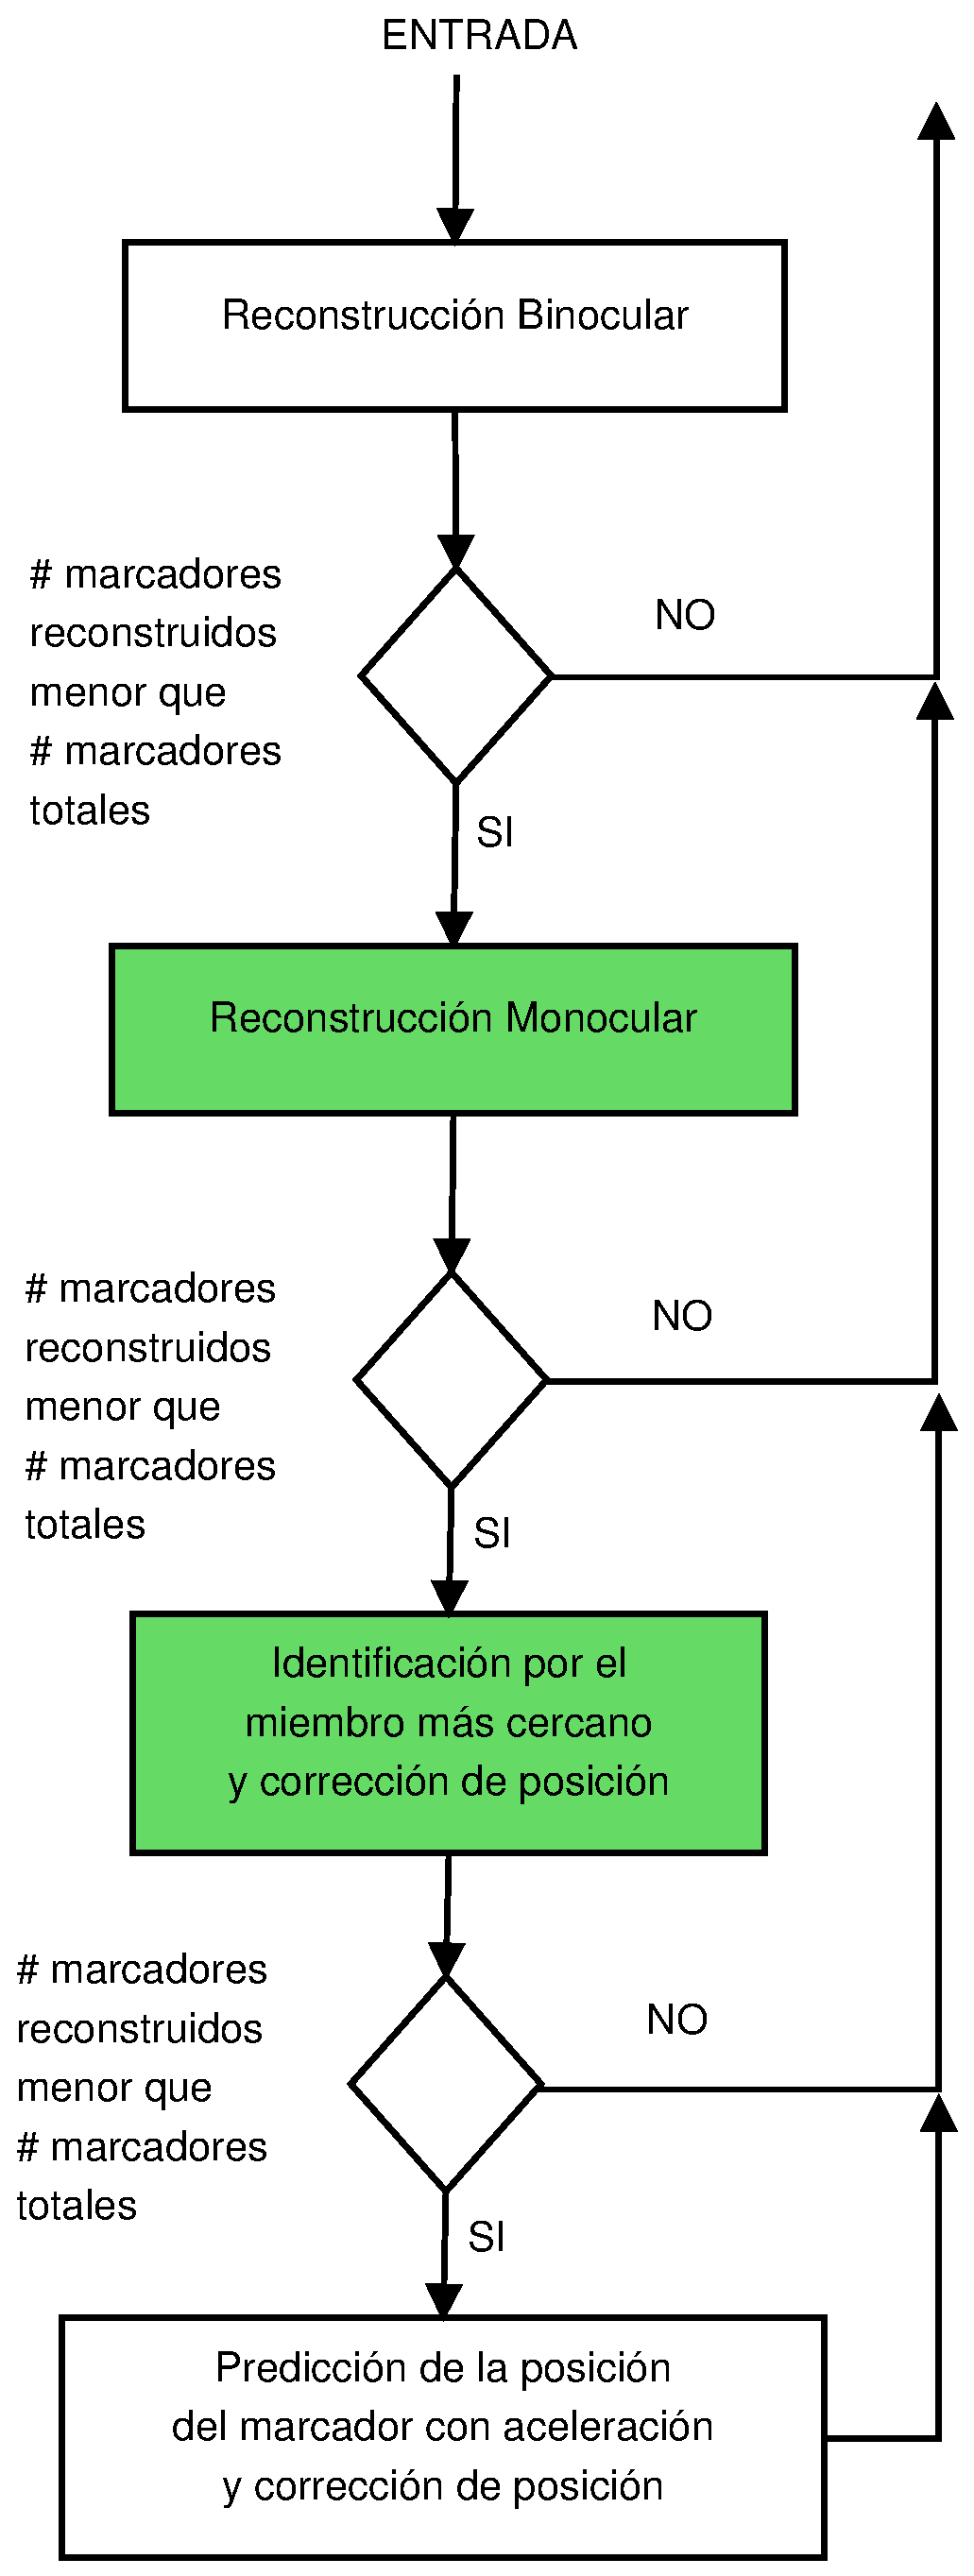
\includegraphics[scale=0.25]{img/Sistema_completo/Diagrama_Detalle.eps}
\end{center}
\caption{Detalle del bloque de corrección.}
\label{fig:bloqCorr}
\end{figure}

Una vez realizada la triangulación estéreo, se verifica que el número de marcadores reconstruidos sea igual a la cantidad de marcadores que efectivamente se estén usando en la adquisición de datos. Si esta condición no se verifica, se ejecuta un “bloque de corrección” para solucionarlo. El “bloque de corrección” a su vez, contiene  varios sub-bloques, los cuales pueden verse en la figura \ref{fig:bloqCorr}.

En primer lugar, se efectúa la reconstrucción de marcadores utilizando \emph{reconstrucción binocular} y \emph{monocular}. Estos métodos son de menor precisión y exigencia que la triangulación estéreo ya que usan dos o una cámara respectivamente en lugar de tres (reconstrucción trinocular).

 Si en la salida de cada uno de los bloques anteriores la condición de todos los marcadores reconstruidos aún no se cumple, se pasa al siguiente bloque, donde se asocian los marcadores 3D reconstruidos que aún no fueron identificados con aquellas articulaciones del modelo de esqueleto ajustado en la inicialización que no tienen ningún marcador asociado. Para esto, se evalúan las distancias de los marcadores no identificados con la posición de las articulaciones del modelo en frames anteriores y se asocian aquellos marcadores que se encuentren a menor distancia a cada una de dichas articulaciones. Al tiempo que se realiza esto, se verifica que la distancia entre marcadores asociados a un mismo hueso del esqueleto se mantenga aproximadamente constante.
 
Por último si aún faltan marcadores sin reconstruirse, se utiliza como último recurso la estimación de la posición del marcador evaluando la aceleración del mismo en frames anteriores y verificando que dicha estimación sea coherente con el modelo de esqueleto.


Hasta acá se tiene la explicación del sistema diseñado. 

No hay que pasar por alto que, si bien se intentó reproducir el sistema propuesto por Herda\cite{herda} tal cual se especificaba en su documentación, se presentaron diversos obstáculos que impidieron poder implementar los bloques de reconstrucción y tracking como se detalló anteriormente. El principal obstáculo fue el calendario, ya que la cantidad de módulos a implementar fue demasiado grande en comparación con el tiempo que se dispuso. Otro factor que influyó, como se mencionó anteriormente, fueron las ambigüedades presentadas en las especificaciones de los bloques en la documentación de Herda\cite{herda}, ya que retrasaron la etapa de estudio del sistema dado que en algunos bloques se tuvo que investigar e implementar métodos para poder superar estos vacíos que se presentaban en la teoría.

 A raíz de esto, se decidió darle prioridad a los bloques principales del diagrama de forma tal de tener implementado un sistema de punta a punta, capaz de capturar la posición 3D de un sujeto realizando el movimiento de marcha a lo largo del tiempo. Estos bloques son:
 \begin{itemize}
 	\item Détección de marcadores
 	\item Triangulación estéreo (Reconstrucción)
 	\item Tracking 3D
 	\item Calibración
 \end{itemize}

En los capítulos que siguen, se explicará el funcionamiento de estos bloques de forma detallada, asi como su implementación y el análisis de resultados.